\chapter{Null geodesics and images in Kerr spacetime}
\label{s:gik}

\minitoc

\section{Introduction}

Having investigated the properties of generic causal geodesics
in Schwarzschild spacetime in Chap.~\ref{s:ges}, we focus here on null
geodesics.


\section{Main properties of null geodesics} \label{s:gik:properties}

We shall distinguish the null geodesics with $E=0$ (the so-called \emph{zero-energy} geodesics,
cf. Sec.~\ref{s:gek:sign_E})
 from those having
$E \neq 0$. Indeed, in the latter case, we will rescale the angular momentum
$L$ and the Carter constant $Q$ by $E$, so that only two constants of motion become
pertinent for the study: $L/E$ and $Q/E^2$.
We thus treat first the particular case $E=0$.

\subsection{Null geodesics with $E=0$}


First, we note that a geodesic $\Li$ with $E=0$ cannot exist outside the ergoregion
$\mathscr{G}$, by virtue of the result (\ref{e:gek:E_positive}). In particular,
it cannot exist far from the black hole.

Another property of null geodesics with $E=0$ is to have a non-negative Carter constant:
\be \label{e:gik:Q_nonneg_E_zero}
   \encadre{ Q \geq 0 }_{E=0} .
\ee
This follows immediately from the result of Sec.~\ref{s:gek:th_motion}
stating that a necessary condition for $Q < 0$ is $a\neq 0$ and
$|E| > \sqrt{\mu^2 + L^2/a^2}$. Specializing this last inequality to $\mu=0$
and $E=0$, we get $0 > |L|$, which is impossible.

Besides, if $\Li$ has some part in $\M_{\rm I}$ (necessarily in the outer ergoregion)
or in $\M_{\rm III}$ (necessarily in the inner ergoregion),
the constraint (\ref{e:gek:future_directed_Carter})
reduces to $L<0$:
\be \label{e:gik:E_zero_L_neg_ergo}
    \Li \cap (\M_{\rm I} \cup \M_{\rm III}) \neq  \varnothing \quad \Longrightarrow \quad L < 0 .
\ee
We shall see below that actually $L \leq 0$ for all zero-energy null geodesics, as soon as $a\neq 0$.

The equations of geodesic motion expressed in terms of the Mino parameter $\lambda'$
[system (\ref{e:gek:eom_Mino})] simplify considerably for a geodesic $\Li$ with $\mu=0$ and $E=0$:
\begin{subequations}
\begin{align}
&  \derd{t}{\lambda'} = - \frac{2 a m L r}{\Delta} \label{e:gik:eom_t_E_zero} \\
&  \derd{r}{\lambda'} = \eps_r \sqrt{ R(r) }  \label{e:gik:eom_r_E_zero}\\
&  \derd{\th}{\lambda'} = \eps_\th \sqrt{\Theta(\th)}  \\
&  \derd{\ph}{\lambda'}  = \frac{L}{\Delta\sin^2\th} \left( r^2 - 2 m r + a^2\cos^2\th \right) ,
                                \label{e:gik:eom_ph_E_zero}
\end{align}
\end{subequations}
with [cf. Eqs.~(\ref{e:gek:R_r_powers}) and (\ref{e:gek:Theta_Q})]:
\be \label{e:gik:R_E_zero}
    R(r) = - (Q+L^2) r^2 + 2m (Q+L^2) r - a^2 Q
\ee
\be \label{e:gik:Theta_E_zero}
    \Theta(\th) = Q - \frac{L^2}{\tan^2\th} .
\ee
By combining (\ref{e:gik:eom_t_E_zero}) and (\ref{e:gik:eom_ph_E_zero}), we get
\be
    \encadre{ \left. \derd{\ph}{t} \right| _{\Li} = \frac{2mr - r^2 - a^2\cos^2\th}{2 a m r\sin^2\th} }_{E=0} .
\ee
It is remarkable that this expression does not depend on $L$ or $Q$; it is therefore the
same for all zero-energy null geodesics. Moreover, we note that the numerator
of the right-hand side is always positive or zero in the closure $\overline{\mathscr{G}}$ of the ergoregion,
which is precisely defined by $2mr - r^2 - a^2\cos^2\th \geq 0$ (cf. Sec.~\ref{s:ker:ergoregion})
and where $\Li$ is necessarily confined. Since moreover $r > 0$ in $\overline{\mathscr{G}}$,
we conclude that
\be
    \left. \derd{\ph}{t} \right| _{\Li} \geq 0 .
\ee




To proceed, we shall distinguish the subcase $Q=0$ from $Q\neq 0$.

\subsubsection{Case $Q=0$}

If the zero-energy null geodesic $\Li$ has a vanishing Carter constant $Q$, Eq.~(\ref{e:gik:Theta_E_zero}) reduces to $\Theta(\th) = -L^2 / \tan^2\th$,
so that the constraint $\Theta(\th) \geq 0$ [Eq.~(\ref{e:gek:Theta_non_neg})]
implies $L=0$ or $\th = \pi/2$ .

In the first case, the four constants of motion $\mu$, $E$, $L$ and $Q$ are
zero. By virtue of the result (\ref{e:gek:all_const_zero}), $\Li$
is nothing but a null geodesic generator of the event horizon $\Hor$ or of the
inner horizon $\Hor_{\rm in}$.

In the second case ($\th=\pi/2$), $\Li$ is confined to the equatorial plane.
If $L=0$, we are back to the first case: $\Li$ is null geodesic generator of $\Hor$ or
$\Hor_{\rm in}$ lying in the equatorial plane.
If $L\neq 0$, the radial motion of $\Li$ is governed by Eq.~(\ref{e:gik:eom_r_E_zero}) with the
expression (\ref{e:gik:R_E_zero}) of $R(r)$ reduced to
\be
    R(r) = L^2 r (2m - r) .
\ee
The constraint $R(r) \geq 0$ [Eq.~(\ref{e:gek:R_non_neg})] implies then
that the motion is within the range $0 \leq r \leq 2 m$, with $r=2m$
being a $r$-turning point, since it is a simple root of $R(r)$ (cf. Sec.~\ref{s:gek:turning_points}).
It corresponds to the outer edge of the ergoregion in the equatorial plane,
cf. Eq.~(\ref{e:ker:r_ergo_p_eq}). Hence we have necessarily $\Li\cap \M_{\rm I} \neq \varnothing$
and (\ref{e:gik:E_zero_L_neg_ergo}) applies: $L < 0$.
The inner boundary of the radial motion, $r=0$, is the ring singularity.

We conclude that
\begin{greybox}
Any null geodesic with $E=0$ and $Q=0$
is either a null generator of one of the two Killing horizons
$\Hor$ or $\Hor_{\rm in}$ (in which case, it has $L=0$) or it has
$L < 0$, lies in the equatorial plane and terminates at the ring singularity,
after possibly a turning point at the outer ergosphere.
\end{greybox}

\subsubsection{Case $Q\neq 0$}

This case actually corresponds to $Q > 0$, since $Q<0$ is forbidden by
(\ref{e:gik:Q_nonneg_E_zero}). We set
\be
    \bar{L} := \frac{L}{\sqrt{Q}}
\ee
and rewrite expression (\ref{e:gik:R_E_zero}) for $R(r)$ as
\be \label{e:gik:R_E_zero_Lb}
    R(r)/Q  = - (1 + \bar{L}^2) r^2 + 2m (1 + \bar{L}^2) r - a^2 .
\ee
Since $1 + \bar{L}^2 \neq 0$, this is a second-order polynomial in $r$,
whose two roots are
\be \label{e:gik:E_zero_rmin_rmax}
    r_{\rm min} = m - \sqrt{m^2 - \frac{a^2}{1 + \bar{L}^2}}
    \qand
    r_{\rm max} = m + \sqrt{m^2 - \frac{a^2}{1 + \bar{L}^2}} .
\ee
Since $m^2 \geq a^2$, the two roots are real. They are distinct
except for $a=m$ and $L=0$.
The range of radial motion being determined by $R(r)\geq 0$
[Eq.~(\ref{e:gek:R_non_neg})], we get
\be
    r_{\rm min} \leq r \leq r_{\rm max} ,
\ee
with a turning point at $r_{\rm min}$ and at $r_{\rm max}$.
Given that $r_- = m - \sqrt{m^2 - a^2}$ and $r_+ = m + \sqrt{m^2 - a^2}$
[Eq.~(\ref{e:ker:def_r_pm})], we note that
\be
     0 \leq r_{\rm min} \leq r_- \leq m \leq r_+ \leq r_{\rm max} \leq 2 m ,
\ee
with $r_{\rm min} = 0$ for $a = 0$ or $\bar{L}^2 \to +\infty$,
$r_{\rm min} = r_-$ for $L=0$, $r_{\rm max} = 2m$ for $a=0$
or $\bar{L}^2 \to +\infty$ and $r_{\rm max} = r_+$ for $L=0$.
If $L\neq 0$ and $a\neq 0$, then $r_{\rm max} > r_+$, so that $\Li$ has a part in the outer
ergoregion and (\ref{e:gik:E_zero_L_neg_ergo}) implies that $L < 0$.
Taking into account the results obtained for $Q=0$, we conclude
that
\begin{greybox}
For $a\neq 0$, any null geodesic with $E=0$ has necessarily
\be
    \encadre{ L \leq 0 }_{{a\neq 0\atop E=0}}.
\ee
\end{greybox}

\begin{remark}
If $L\neq 0$, the limit $\bar{L}^2 \to +\infty$ corresponds to $Q\to 0$
and we recover the range $[0, 2m]$ determined above in the case $Q=0$.
\end{remark}

Let us consider a zero-energy null geodesic $\Li$ emitted outward (i.e.
with $\epsilon_r = +1$) from a point $A$ in the outer ergoregion $\mathscr{G}^+$.
The coordinate $r$ increases along $\Li$ from $r_A$ to $r_{\rm max}$, which
corresponds to a $r$-turning point. Then $r$ decreases to $r_+$, which means
that $\Li$
crosses the black hole event horizon $\Hor$ and enters the region $\M_{\rm II}$.
In all $\M_{\rm II}$, $r$ keeps decreasing and reaches $r_-$. There $\Li$
crosses the inner horizon $\Hor_{\rm in}$ and enters the region $\M_{\rm III}$,
where $r$ continues to decrease until it reaches $r_{\rm min}$. The latter
corresponding to a $r$-turning point, $r$ starts to increase and reaches
$r_-$ again. There one might think that $\Li$ crosses the inner horizon
$\Hor_{\rm in}$ and enters into $\M_{\rm II}$. But this is impossible since
$\Hor_{\rm in}$ is a 1-way membrane: it can be crossed by a causal curve
from $\M_{\rm II}$ to $\M_{\rm III}$ but not in the reverse way. Moreover, $r$
could not continue to increase into $\M_{\rm II}$ since $r$ must be decreasing
towards the future in all this region (this follows from the hypersurfaces
$r=\mathrm{const}$ being spacelike in $\M_{\rm II}$, cf. Sec.~\ref{s:ker:Killing_hor}).
The solution to this apparent puzzle is immediate as soon as one realizes
that the boundary $r = r_-$ of $\M_{\rm III}$ is not entirely constituted
by $\Hor_{\rm in}$: it also comprises a null hypersurface that separates
$\M_{\rm III}$ from a region distinct from $\M_{\rm II}$ in
the maximally extended Kerr spacetime, cf. Fig.~\ref{f:ker:max_ext}. This region
is a ``time-reversed'' copy of $\M_{\rm II}$ and is
denoted by ${\M_{\rm II}^*}'$ in Fig.~\ref{f:ker:max_ext} (cf. Sec.~\ref{s:ker:max_extension}
for details).
So actually, when it reaches $r=r_-$, the null geodesic $\Li$ enters
${\M_{\rm II}^*}'$. There $r$ necessarily increases towards the future, at
the opposite of $\M_{\rm II}$. It reaches then $r=r_+$, where $\Li$
crosses a white hole\index{white hole} horizon and emerges into
the asympototically flat region $\M_{\rm I}''$, as illustrated in
Fig.~\ref{f:gik:zero_ener_traj}. The region $\M_{\rm I}''$ is similar
to $\M_{\rm I}$. In particular, $\Li$ is confined into the outer ergoregion
of $\M_{\rm I}''$, having a $r$-turning point at $r=r_{\rm max}$ (same value
(\ref{e:gik:E_zero_rmin_rmax}) as in $\M_{\rm I}$). Then a new cycle
begins, with $\Li$ entering the future event horizon of $\M_{\rm I}''$.

\begin{figure}
\centerline{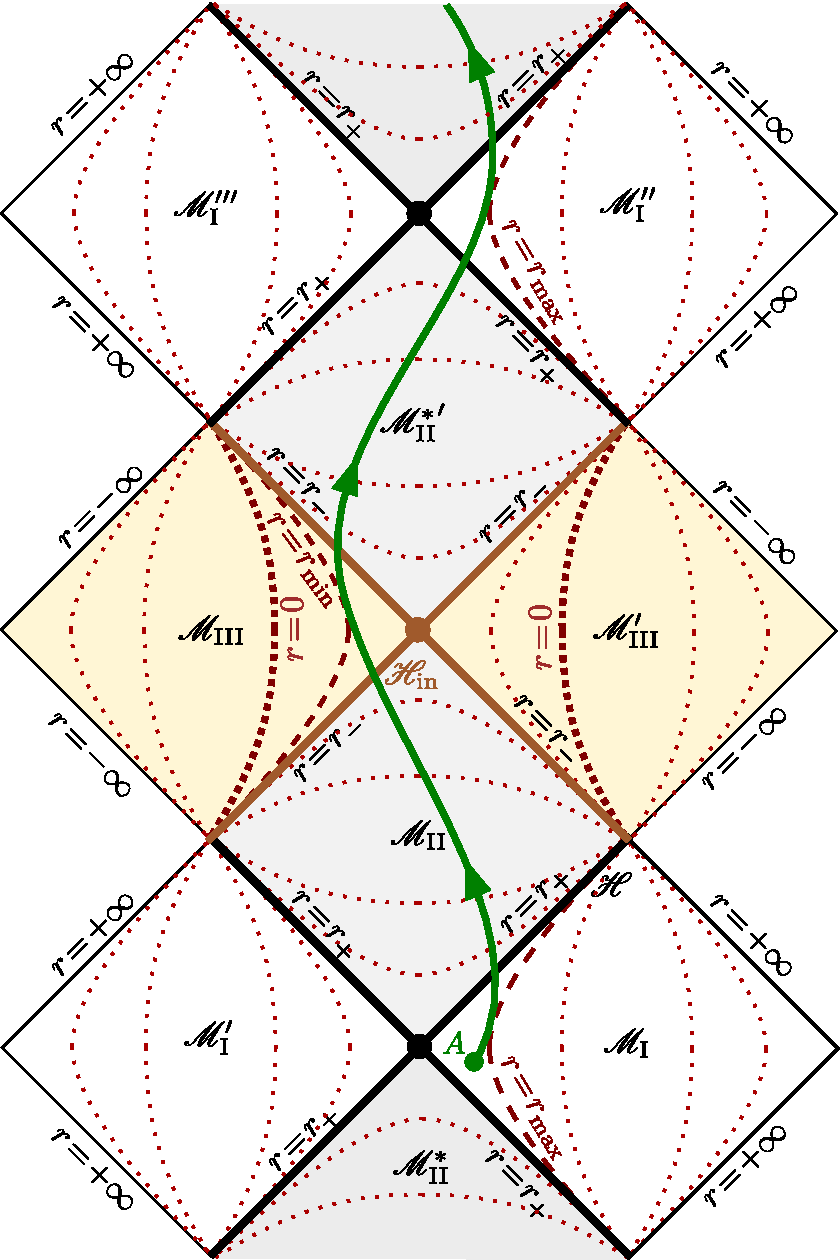
\includegraphics[width=0.6\textwidth]{gik_zero_ener_traj.pdf}}
\caption[]{\label{f:gik:zero_ener_traj} \footnotesize
Trajectory in the extended Kerr spacetime of a null geodesic
with $E=0$, $Q>0$ and $L<0$, emitted from a point $A$ in the outer ergoregion.
}
\end{figure}

The $\theta$-motion of $\Li$ is constrained by $\Theta(\th) \geq 0$ [Eq.~(\ref{e:gek:Theta_non_neg})],
which, given expression~(\ref{e:gik:Theta_E_zero}) for $\Theta$, is
equivalent to
\be
    \th_{\rm min} \leq \th \leq \pi - \th_{\rm min} \quad\mbox{with}\quad
    \th_{\rm min} := \arctan (-\bar{L}) .
\ee
For $L = 0$, one has $\th_{\rm min} = 0$, so that $\th$ takes all values in the
range $[0,\pi]$, which means that $\Li$
crosses repeatedly the rotation axis. For $L< 0$, one has $0 < \th_{\rm min} < \pi/2$ and
$\Li$ oscillates symmetrically about the equatorial plane,
having two $\th$-turning points, at $\th_{\rm min} $ and $\pi-\th_{\rm min}$. Of course, we
recover the general results for $Q>0$ of Sec.~\ref{s:gek:th_motion}.

We can obtain $r$ as a function of $\th$ along $\Li$ by evaluating the integrals
in the identity (\ref{e:gek:integr_Mino}):
\[
    \dashint_{r_0}^r \frac{\eps_r \, \D \bar{r}}{\sqrt{R(\bar{r})}}
   = \dashint_{\th_0}^\th \frac{\eps_\th \, \D \bar{\th}}{\sqrt{\Theta(\bar{\th})}}
\]
Using (\ref{e:gik:R_E_zero_Lb}) and (\ref{e:gik:Theta_E_zero}), we get on
any portion of $\Li$ where $\eps_r$ and $\eps_\th$ are constant,
\[
    \eps_r \int_{r_0}^r
    \frac{\D \bar{r}}{\sqrt{- (1 + \bar{L}^2) \bar{r}^2 + 2m (1 + \bar{L}^2) \bar{r} - a^2}}
    = \eps_\th \int_{\th_0}^\th \frac{\D \bar{\th}}{\sqrt{1 - \bar{L}^2/\tan^2\bar{\th}}} .
\]
The changes of variables
\[
    x = \frac{r/m - 1}{\sqrt{1 - \frac{a^2}{m^2(1 + \bar{L}^2)}}}
    \qand
    \mu = \cos\th
\]
lead to
\[
   \frac{\eps_r}{\sqrt{1 + \bar{L}^2}} \int_{x_0}^x \frac{\D\bar{x}}{\sqrt{1 - \bar{x}^2}}
   = - \eps_\th \int_{\cos\th_0}^{\cos\th} \frac{\D\mu}{\sqrt{1 - (1 + \bar{L}^2)\mu^2}} .
\]
The integration is then immediate:
$\arcsin x = - \eps_r \eps_\th \arcsin(\sqrt{1 + \bar{L}^2} \cos\th) + K$,
where $K$ is a constant, from which we get
\be \label{e:gik:E_zero_r_theta}
   \encadre{ r = m + m\sqrt{1 - \frac{a^2}{m^2(1 + \bar{L}^2)}} \; \sin \left[
        K - \eps_r \eps_\th \arcsin\left(\sqrt{1 + \bar{L}^2} \cos\th\right) \right] }.
\ee
Since $\sqrt{1 + \bar{L}^2} \cos\th_{\rm min} = 1$, we see that the constant
$K$ is related to the value of $r$ at $\th = \th_{\rm min}$ by
\be \label{e:gik:E_zero_K}
    K =  \arcsin \left( \frac{r(\th_{\rm min})/m - 1}{\sqrt{1 - \frac{a^2}{m^2(1 + \bar{L}^2)}}} \right)
    + \eps_r \eps_\th \frac{\pi}{2} .
\ee
Note that $K$ is not a constant all along $\Li$, but only on portions where
$\eps_r$ and $\eps_\th$ are constant.
Expression~\ref{e:gik:E_zero_r_theta} gives the trace of the zero-energy
null geodesic $\Li$ in a meridional plane. It depends on $Q$ and $L$ only
through the ratio $\bar{L} := L / \sqrt{Q}$. It depends as well on the value of
$r$ at $\th_{\rm min}$ via $K$, as it appears in Eq.~(\ref{e:gik:E_zero_K}).
An example is shown in Fig.~\ref{f:gik:zero_ener_merid} for $a/m = 0.9$, $L / \sqrt{Q} = -1$
and $r(\th_{\rm min}) = 1.5\, m$. It has $\th_{\rm min} = \pi/4$,
$r_{\rm min} \simeq 0.229\, m$ and $r_{\rm max} \simeq 1.771\, m$,
while for $a/m = 0.9$, one has $r_- \simeq 0.564\, m$ and $r_+ \simeq 1.436\, m$.

\begin{figure}
\centerline{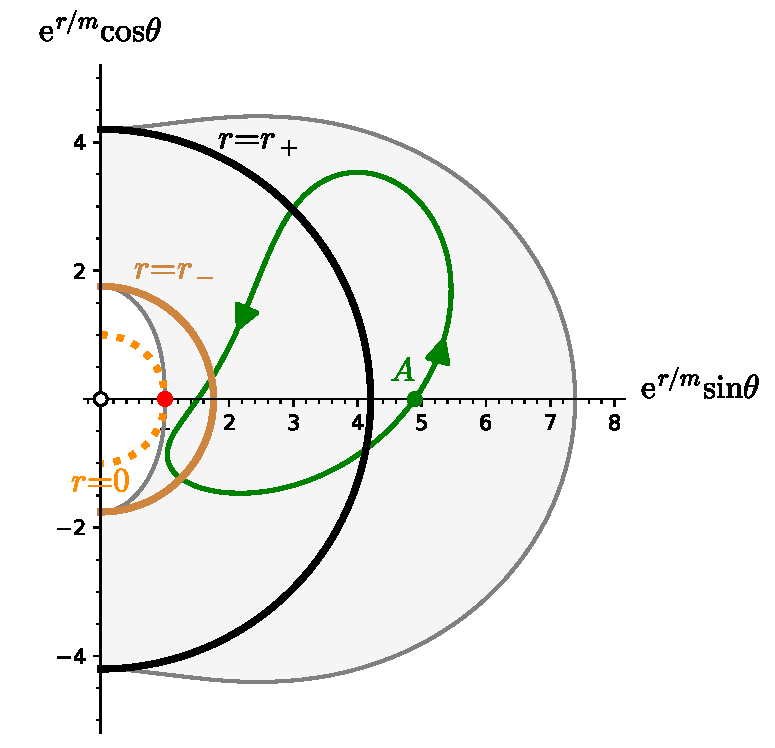
\includegraphics[width=0.7\textwidth]{gik_zero_ener_merid.pdf}}
\caption[]{\label{f:gik:zero_ener_merid} \footnotesize
Trajectory in the meridional plane of a null geodesic (green curve)
with $E=0$, $Q>0$, $L = - \sqrt{Q}$ and $r(\th_{\rm min}) = 1.5 \, m$
in a Kerr spacetime with $a/m = 0.9$.
The meridional plane is described in terms of
O'Neill exponential coordinates $x = \mathrm{e}^{r/m}\sin\th$ and $z = \mathrm{e}^{r/m}\cos\th$,
as in Figs.~\ref{f:ker:ergo_a90} -- \ref{f:ker:ergo_a99}.
The dotted orange circle marks the locus of $r=0$, with the
two red dots marks indicating the curvature singularity at $r=0$ and $\th=\pi/2$.
The ergoregion is shown in grey. The area $\rm I$ is defined by $r> r_+$ and
correspond to the regions denoted by $\M_{\rm I}$ and $\M_{\rm I}''$ in Fig.~\ref{f:gik:zero_ener_traj},
the area $\rm II$ is defined by $r_- < r < r_+$ and
correspond to the regions denoted by $\M_{\rm II}$ and ${\M_{\rm II}^*}'$  in Fig.~\ref{f:gik:zero_ener_traj} and the area $\rm III$ is defined by $r < r_-$ and
correspond to the region denoted by $\M_{\rm III}$ in Fig.~\ref{f:gik:zero_ener_traj}.
}
\end{figure}


\subsection{Equations of geodesic motion for $E\neq 0$}


\subsection{$\theta$-motion}

Specializing the general results of Sec.~\ref{s:gek:th_motion} to $\mu=0$, we
get
\begin{greybox}
\begin{itemize}
\item A null geodesic $\Li$ of Kerr spacetime cannot encounter the rotation axis unless it has $L=0$.
\item If $a=0$ (Schwarzschild limit) or $|E| \leq |L|/a$,
the Carter constant $Q$ is necessarily non-negative:
\be \label{e:gik:Q_nonnegative}
    Q \geq 0 .
\ee
\item The Carter constant $Q$ can take negative values only if
$a\neq 0$ and $|E| > |L|/a$; its range is then
limited from below:
\be
    Q \geq Q_{\rm min} = - \left( a |E| - |L| \right) ^2.
\ee
If $Q<0$, $\Li$ is called a \defin{vortical null geodesic}\index{vortical geodesic}; it
never encounters the equatorial plane.
\item If $Q>0$ and $L\not=0$, $\Li$ oscillates symmetrically about the equatorial plane,
between two turning points, $\th_0$ and $\pi-\th_0$, such that $0<\th_0<\pi/2$.
If $Q>0$ and $L=0$, $\Li$
crosses repeatedly the rotation axis, with $\th$ taking all values in the
range $[0,\pi]$.
\item If $Q=0$, $\Li$ is stably confined to the equatorial plane
for $a |E|  < |L|$ or $a |E|  = |L| \neq 0$;
for $a |E| > |L|$, $\Li$ either lies unstably in the equatorial
plane or approaches it asymptotically from one side, while for $L=0$ and ($a=0$ or $|E|=\mu$),
$\Li$ lies at a constant value $\th=\th_0\in[0,\pi]$.
\item If $Q_{\rm min} < Q < 0$, $\Li$ oscillates between two turning
points strictly located in the Northern hemisphere ($0<\th<\pi/2$) or in
the Southern hemisphere ($\pi/2<\th<\pi$) for $L\neq 0$, while for $L=0$,
$\Li$ oscillates about the rotation axis, without encoutering the equatorial
plane, having a turning point at $\th_0$ such that $0<\th_0<\pi/2$
(motion in the Northern hemisphere) or $\pi/2<\th_0<\pi$
(motion in the Southern hemisphere).
\item If $Q = Q_{\rm min}$, $\Li$ lies stably at a constant value $\th=\th_0$,
with $\th_0 = 0$ or $\pi$ (the rotation axis) for $L=0$ and $0<\th_0< \pi/2$
or $\pi/2<\th_0<\pi$ for $L\neq 0$.
\end{itemize}
\end{greybox}


\section{Principal null geodesics}

\section{Photon region}

\subsection{Spherical null geodesics}

\section{Images}
